\documentclass[a4paper]{article}
\usepackage{amsfonts}
\usepackage{amsmath}
\usepackage{amssymb}
\usepackage{graphicx}
\usepackage{extarrows}

\newcommand{\limit}{\lim\limits}

\begin{document}

\noindent \large Auteur: Seda Jusjajeva\\
\noindent \large Studierichting: Informatica\\
\noindent \large Oefeningenreeks 3G nr. 18.2 \\

\medskip

\normalsize


$f(x) = \sqrt{\dfrac{x}{x + 1}}$ \\

$\operatorname{dom}f = \mathbb{R} \setminus [-1,0[ $ \\

Nulpunten: $x = 0$ \\

Polen: $x + 1 = 0 \Leftrightarrow x = -1$ \\

VA: \\

$\limit_{x\to-1+} \sqrt{\dfrac{x}{x + 1}} = \dfrac{-1}{0^+} = -\infty$ \\

$\limit_{x\to-1-} \sqrt{\dfrac{x}{x + 1}} = \dfrac{-1}{0^-} = +\infty$ \\

$\Rightarrow x = -1$\\

HA: \\

$\limit_{x\rightarrow \infty} \sqrt{\dfrac{x}{x+1}} = \dfrac{\infty}{\infty} $\\

$= \limit_{x \to \infty} \sqrt{\dfrac{\dfrac{x}{x}}{\dfrac{x}{x} + \dfrac{1}{x}}} = \limit_{x \to \infty} \sqrt{\dfrac{1}{1 + \dfrac{1}{x}}}$ \\

$= \sqrt{\dfrac{1}{1 + 0}} = \sqrt{1} = 1$ \\

$\Rightarrow y = 1$.\\

$\begin{array}{r|ccccccc}
    x    & -\infty &   & -1 &     & 0 &   & +\infty \\ 
    \hline
    f(x) &         & + & |  & /// & 0 & + &\\ 
\end{array}$ \\

De functie ligt naar $-\infty$ boven de HA en naar $+\infty$ onder de HA. \\

SA: \\

geen SA. \\

Tekenonderzoek: \\

$f'(x) = \dfrac{d}{dx}\left(\sqrt{\dfrac{x}{x + 1}}\right)$ \\

$= \dfrac{1}{2} \left(\dfrac{x}{x+1}\right)^{-\tfrac{1}{2}} \cdot \dfrac{d}{dx}\left(\dfrac{x}{x+1}\right)$ \\

$= \dfrac{1}{2} \left(\dfrac{x}{x+1}\right)^{-\tfrac{1}{2}} \cdot  \dfrac{1 \cdot (x+1) - x \cdot 1}{(x+1)^2}$ \\

$= \dfrac{1}{2} \left(\dfrac{x}{x+1}\right)^{-\tfrac{1}{2}} \cdot \dfrac{x + 1 - x}{(x+1)^2}$ \\

$= \dfrac{1}{2} \left(\dfrac{x}{x+1}\right)^{-\tfrac{1}{2}} \cdot \dfrac{1}{(x+1)^2}$ \\

$= \dfrac{1}{2} \sqrt{\dfrac{x+1}{x}} \cdot \dfrac{1}{(x+1)^2}$ \\

$= \dfrac{\sqrt{x+1}}{2\sqrt{x} \cdot (x+1)^2}$ \\

$= \dfrac{1}{2\sqrt{x} \cdot (x+1)^{\tfrac{3}{2}}}$ \\

$f''(x) = \dfrac{d}{dx}\left(\dfrac{1}{2\sqrt{x} \cdot (x + 1)^{\tfrac{3}{2}}}\right)$ \\

$= \dfrac{1}{2} \cdot \dfrac{d}{dx}\left(\dfrac{1}{\sqrt{x} \cdot (x + 1)^{\tfrac{3}{2}}}\right)$ \\

$= \dfrac{1}{2} \cdot \left( -\dfrac{1}{\left(\sqrt{x}(x+1)^{\tfrac{3}{2}}\right)^2} \cdot \dfrac{d}{dx}\left(\sqrt{x}\left(x+1\right)^{\tfrac{3}{2}}\right) \right)$ \\

$= \dfrac{1}{2} \cdot \left( -\dfrac{1}{x(x+1)^3} \cdot \left( \dfrac{d}{dx}\sqrt{x}\left(x+1\right)^{\tfrac{3}{2}} + \sqrt{x}\dfrac{d}{dx}\left(x+1\right)^{\tfrac{3}{2}} \right) \right)$ \\

$= \dfrac{1}{2} \cdot \left( -\dfrac{1}{x(x+1)^3} \cdot \left( \dfrac{(x+1)^{\tfrac{3}{2}}}{2\sqrt{x}} + \dfrac{3\sqrt{x}(x+1)^{\tfrac{1}{2}}}{2} \right) \right)$ \\

$= \dfrac{1}{2}\cdot\left(\left( -\dfrac{1}{x(x+1)^{3}} \cdot \dfrac{(x+1)^{\tfrac{3}{2}}}{2\sqrt{x}} \right) + \left( -\dfrac{1}{x(x+1)^3} \cdot \dfrac{3\sqrt{x}(x+1)^{\tfrac{1}{2}}}{2} \right)\right)$ \\

$= \dfrac{1}{2}\cdot \left(\left( -\dfrac{1}{2x^{\tfrac{3}{2}}(x+1)^{\tfrac{3}{2}}} \right) + \left( -\dfrac{3}{2x^{\tfrac{1}{2}}(x+1)^{\tfrac{5}{2}}}\right)\right)$ \\

$= \dfrac{1}{2}\cdot \left( \dfrac{-(x+1)-3x}{2x^{\tfrac{3}{2}}(x+1)^{\tfrac{5}{2}}} \right)$ \\

$= -\dfrac{4x + 1}{4x^{\tfrac{3}{2}}(x+1)^{\tfrac{5}{2}}}$ \\

$\begin{array}{r|ccccc}
  x      &          & -1 &     & 0 & \\ 
  \hline
  f(x)   & +        & |  & /// & 0 & + \\
  f'(x)  & +        & |  & /// & | & + \\
  f''(x) & +        & |  & /// & | & - \\ 
  \hline
  f(x)   & \nearrow &    &     &   & \nearrow \\
         & \smile   &    &     &   & \frown \\
\end{array}$ \\



Grafiek: \\

\begin{figure}[h]
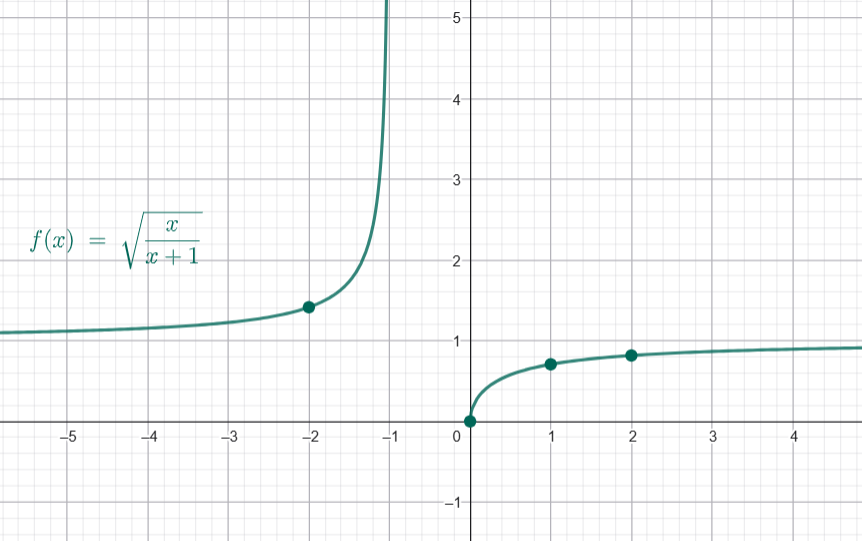
\includegraphics[width=\linewidth]{3G-18.2-seda.jusjajeva.INF.png} \\
\end{figure} 


\begin{thebibliography}{999}
%\bibitem{a} Referentie
\end{thebibliography}
\end{document}